%%%%%%%%%%%%%%%%%%%%%%%%%%%%%%%%%
% 9 sept 2013 [Jan]: opm. van Inge verwerkt
%
% 14/9/11 [Jan]: enkele typfouten verbeterd, bad boxes eruit gehaald
%
% 23/05/11 [Greetje]: figuren geüdate, links aangepast en wat tekst aangepast
%
% 15/9/04 [Jan]: aanvulling constructies Greet
%
% 6/9/04 [Jan]: tekst aangemaakt.
%%%%%%%%%%%%%%%%%%%%%%%%%%%%%%%%%

\chapter{Passer en Liniaal (P.e.L.)}
\begin{quote}
     \textit{{\small Nu begon de Rode Koningin weer. `Kun je nuttige
     vragen beantwoorden?' zei ze. 'Hoe wordt brood gemaakt?'}}

     \textit{{\small `\emph{Dat} weet ik!' riep Alice gretig. `Je
     neemt een hoeveelheid bloem--'}}

     \textit{{\small `Waar pluk je de bloem?' vroeg de Witte Koningin.
     `In een tuin of in het wild?'}}

     \textit{{\small `Maar die wordt helemaal niet \emph{geplukt},'
     legde Alice uit, `die wordt \emph{gemalen}--'}}

     \textit{{\small `Hoeveel malen wordt de bloem gemalen?' zei de
     Witte Koningin. `Laat toch niet zoveel dingen weg.'}}

          Uit `Achter de spiegel' -- Lewis Carroll
\end{quote}

\newpage
\section{Inleiding}
Deze tekst geeft je een kort overzicht van het basisgebruik van `Passer en Liniaal' (kort: `P.e.L.'). In een overzicht op papier gaat echter wel een van de basisprincipes van dit soort van software verloren, met name het dynamisch karakter van constructies. In plaats van een constructie waar je punten kan verslepen, hou je enkel een statische figuur over.

We vinden het toch zinvol om je deze tekst mee te geven. Via een uitgewerkt eenvoudig voorbeeld tonen we je de meest voorkomende acties in P.e.L. Hier staat met andere woorden het  programma centraal en niet de meetkunde die we ermee zullen bedrijven. Voor de meetkundige toepassingen verwijzen we naar de site \url{http://car.rene-grothmann.de/doc_en/index.html}, naar de site van het vak wiskunde (\url{http://wiskunde.khleuven.be}) en het elektronisch leerplatform Toledo.

\section{Downloaden - installeren}
Je downloadt het programma van de hierboven vermelde site. Afhankelijk van je besturingssysteem (Windows, Mac, Linux) zijn er verschillende mogelijkheden om het te installeren. Het programma werkt in principe op elk besturingssysteem, op voorwaarde dat er een versie van Java aanwezig is op je computer. De software is volledig open en gratis. Je kan de broncode bekijken en aanpassen als je dat zou willen.

P.e.L.\ herkent je systeeminstellingen en gebruikt de passende taal (indien aanwezig). Maar zelfs als je een anderstalig systeem hebt, blijft het mogelijk om P.e.L.\ op te starten met Nederlandse menu's en helpsysteem.

Alle technische details vind je  op de site van de auteur van het programma (\url{http://car.rene-grothmann.de/doc_en/index.html})

\section{Het scherm}
Figuur~\ref{fig:PeLscherm} toont het opstartscherm. 
\begin{figure}[htb]
    \centering
    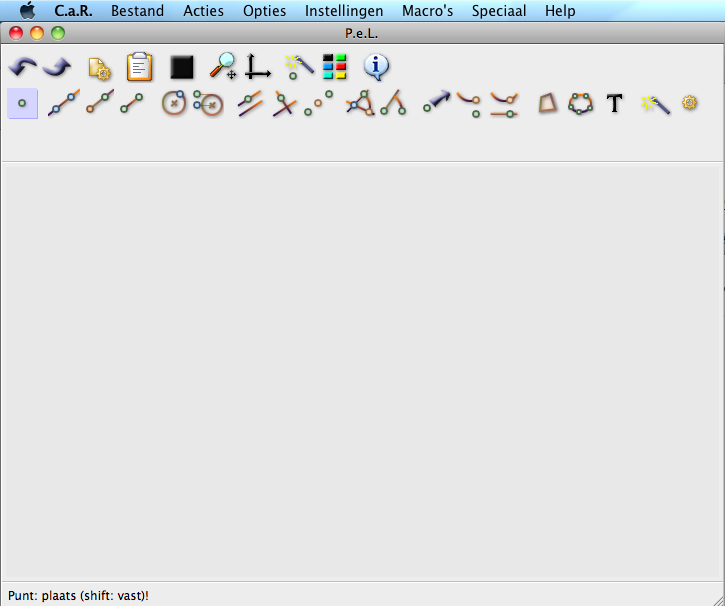
\includegraphics[width=\textwidth]{figuren/PeL/PeLscherm.png}
       \caption{Basisscherm van P.e.L.\ v9.5 met beperkte set werktuigiconen.}
    \label{fig:PeLscherm}
\end{figure}
Je kan vier delen onderscheiden (van boven naar onder\footnote{Het is ook mogelijk om de iconenbalk onder het tekenvenster te zetten. Deze instelling kies je via de opties.}):
\begin{enumerate}
\item Programmamenu's;
\item de iconenbalk;
\item het tekenvenster;
\item de statusbalk.
\end{enumerate}
We merken op dat de iconenbalk een \emph{beperkt aantal iconen} toont. Er zijn er zeker dubbel zoveel. We werken met de `beperkte set werktuigiconen' (aan te vinken in het programmamenu bij `Instellingen'). Je krijgt dan enkel de meest voorkomende iconen te zien. Het is een goed idee om eerst een tijdje te wennen aan de beperkte set iconen en deze dan verder aan te vullen (via `Instellingen') als je vertrouwd bent met het programma. Je kan trouwens alles in P.e.L.\ uitvoeren zonder iconen, via de gewone menu's of via  sneltoetsen (`shortcuts').

Het tekenvenster is de plaats waar de constructie vorm krijgt. Soms kan het nodig zijn om eerst te klikken in dit venster, zodat het \emph{in focus} komt.

De statusbalk is de plaats waar het programma aan de gebruiker laat weten wat het als invoer verwacht \footnote{In de zogenaamde \emph{beschrijvende modus} doet dit vak dienst als invoervak. Meer over deze (snelle) manier van werken vind je op http://wiskunde.khleuven.be}. 

\section{Een voorbeeld}
\subsection{Middelloodlijnen van een driehoek construeren}
We werken stapsgewijs volgende opgave uit: 
\begin{quote}
Construeer de middelloodlijnen van een willekeurige driehoek. 
\end{quote}
Als de constructie klaar is, gaan we op zoek naar een eigenschap van deze drie middelloodlijnen door \'{e}\'{e}n van de punten van de driehoek te verplaatsen.

We gebruiken dit voorbeeld om een aantal principes te illustreren. Een grafisch hoogstaand eindresultaat is iets minder onze bekommernis\footnote{Bij een `echte' constructie moet de grafische kwaliteit \emph{wel} een belangrijk streefdoel zijn. Lijndikte, kleur, benaming, puntsoorten,... kunnen allemaal bijdragen om de constructie zo duidelijk en aantrekkelijk mogelijk te maken.}.

\subsection{Constructie van drie punten}
Alle softwareprogramma's voor dynamische meetkunde hebben met elkaar gemeen dat je eerst een \emph{constructiewerktuig} moet selecteren. Het geselecteerde gereedschap verwacht dan bepaalde invoer van de gebruiker.

Ook punten moet je `construeren'. Kies het puntwerktuig\footnote{We gaan even uit van de veronderstelling dat dit werktuig niet het huidig geselecteerde werktuig is. Het geselecteerde werktuig heeft in de iconenbalk een donkergrijze achtergrond.}. Dat kan op drie manieren:
\begin{enumerate}
\item Klik op het icoon van het puntwerktuig;
\begin{figure}[htb]
    \centering
    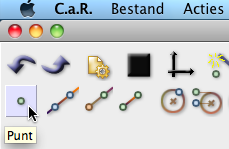
\includegraphics[]{figuren/PeL/Punticoon.png}
       \caption{Selectie via het icoon}
    \label{fig:punticoon}
\end{figure}
\item kies via het menu \texttt{Acties$\rightarrow$Punten$\rightarrow$Punt};
\begin{figure}[htb]
    \centering
    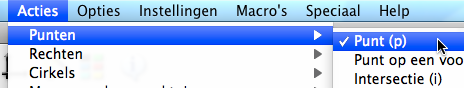
\includegraphics[scale=0.5]{figuren/PeL/Puntmenu.png}
       \caption{Selectie via het menu}
    \label{fig:puntmenu}
\end{figure}
\item De meeste werktuigen hebben een sneltoets. In het menu (zie puntje 2 hierboven) vind je als sneltoets de `p' voor punt\footnote{Meestal is de sneltoets de eerste letter van de Nederlandse benaming van het werktuig, bvb.\ `r' voor rechte, `l' voor lijnstuk, `i' voor intersectie,...}. 
\end{enumerate}
 
Na de selectie staat het icoontje van het puntwerktuig met een donkergrijze achtergrond in de iconenbalk. Het eerste wat je dan doet is de tekst in het statusvenster (onderaan) bekijken. Hier geeft P.e.L.\ aan wat er als invoer verwacht wordt. Bvb.\ in het geval van een punt, staat er `Punt: plaats (Shift: vast)!'. Deze cryptische omschrijving kan je vertalen als: ``Je hebt het puntwerktuig geselecteerd. Ik verwacht nu dat je ergens in het tekenvenster een punt plaatst met de muis. Als je de Shift-toets ingedrukt houdt terwijl je het punt plaatst, maak je een vast punt dat niet meer kan verplaatst worden''. 

Construeer nu drie verschillende punten.

\subsection{Lijnstukken}
Om een driehoek te maken, moet je de drie punten verbinden met lijnstukken. Hiervoor bestaat er een apart werktuig: het \emph{lijnstukwerktuig}. Net zoals bij het puntwerktuig zijn er drie manieren om het te selecteren:
\begin{enumerate}
\item Klik op het icoon van het lijnstukwerktuig;
\begin{figure}[htb]
    \centering
    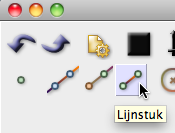
\includegraphics[]{figuren/PeL/Lijnstukicoon.png}
       \caption{Icoon voor lijnstukwerktuig}
    \label{fig:lijnstukicoon}
\end{figure}
\item kies via het menu \texttt{Acties$\rightarrow$Rechten$\rightarrow$Lijnstuk};
\item gebruik de sneltoets `l'. 
\end{enumerate}

Na de selectie van dit werktuig verandert de tekst in het statusvenster in `Lijnstuk: eerste punt?' P.e.L.\ verwacht dat je het eerste punt van het lijnstuk aanduidt. Ga naar \'{e}\'{e}n van de punten met de muis. Als je dicht genoeg in de buurt van het punt met de muisaanwijzer gaat staan, verandert het punt van kleur. Dit betekent dat P.e.L.\ dit punt herkent als een geldige kandidaat. Klik op het punt om het te selecteren. 

Je kan ook klikken op een \emph{vrije ruimte}. P.e.L.\ zal opmerken dat je niet in de buurt van een bestaand punt geklikt hebt en een nieuw punt aanmaken op de plaats waarop je klikte. Opgelet: dit een belangrijke bron van fouten! Meer dan eens gebeurt het dat je denkt op een bestaand punt geklikt te hebben, maar dat je in feite het punt net miste door het onnauwkeurig aan te wijzen.  P.e.L.\ plaatst dan een nieuw punt heel dichtbij het punt dat je eigenlijk wou aanwijzen. Daarom deze raad: \emph{wacht altijd tot het punt dat je wil aanduiden van kleur verandert}. Pas dan ben je zeker dat P.e.L.\ het herkent als een punt dat kan gekozen worden voor het huidige werktuig.

Als alles in orde is verandert de tekst in het statusvak nu in `Lijnstuk: tweede punt (Shift: vaste lengte)?' Vertaling in het Nederlands: ``We werken nog steeds met het lijnstukwerktuig. Duid nu een tweede punt aan als eindpunt voor het lijnstuk. Als je de Shift-toets ingedrukt houdt bij het selecteren van een tweede punt, krijg je een speciaal lijnstuk met vaste grootte''. Op deze voorwerpen met een vaste grootte komen we later terug.

Duid het tweede punt aan (wacht op kleurverandering) en klik met de muis. Het lijnstuk wordt geconstrueerd. Merk op dat de tekst in het statusvak terug verandert naar de tekst van daarnet (eerste punt). \emph{Zolang je geen ander werktuig kiest, blijft het huidige werktuig van kracht}. Construeer nu de andere lijnstukken, tot de driehoek af is.

\subsection{Eigenschappen van een werktuig}
Elk voorwerp dat je construeert wordt bewaard met een aantal standaardeigenschappen, zoals kleur, lijndikte, zichtbaarheid, benaming, grootte,\dots\  Er zijn twee manieren om die eigenschappen te veranderen:
\begin{enumerate}
\item Het gemakkelijkste is dat je \emph{op voorhand} (v\'{o}\'{o}r de constructie van het voorwerp) nadenkt over de gewenste kleur, lijndikte,... en die standaardwaarden aanpast. Deze manier van werken illustreren we in een volgend puntje.
\item Het is echter ook mogelijk om de eigenschappen van een reeds geconstrueerd voorwerp \emph{achteraf} te wijzigen. Ook dit kan op verschillende manieren:
\begin{enumerate}
\item Klik op het icoon van het `wijzigwerktuig' 
\includegraphics[width=0.75cm]{figuren/PeL/wijzigwerktuigicoon.png}. Opgelet: dit icoon krijg je niet te zien in de beperkte set werktuigiconen. Om ook dit icoon te kunnen kiezen, moet je deze instelling eerst uitschakelen. Dit kan via het menu: \\ \texttt{Instellingen$\rightarrow$beperkte set werktuigiconen}.
\item Kies via het menu \texttt{Acties$\rightarrow$Wijzig laatste voorwerp}. Zoals de omschrijving het aangeeft, kan je hiermee \emph{enkel het voorwerp dat je net construeerde}, wijzigen.
\item De snelste manier om de eigenschappen van een voorwerp te wijzigen is rechtsklikken\footnote{Op Mac wordt dat Command (appeltje-toets) + klikken als je maar over \'{e}\'{e}n muisknop beschikt.} op het voorwerp 
\end{enumerate}

\end{enumerate}

Laten we de eigenschappen van een punt bekijken. Klik met de rechtermuisknop op \'{e}\'{e}n van de punten. Er opent een venstertje met een aantal iconen en vakken waarin tekst of getallen ingevuld zijn. Figuur~\ref{fig:punteig} toont dit eigenschappendialoogvenster. Per voorwerp is dit venster licht verschillend (een rechte heeft bvb.\ een paar andere eigenschappen dan een cirkel), maar de basisstructuur is altijd hetzelfde. Daarom bekijken we dit voorbeeld meer in detail.

\begin{figure}[htb]
    \centering
    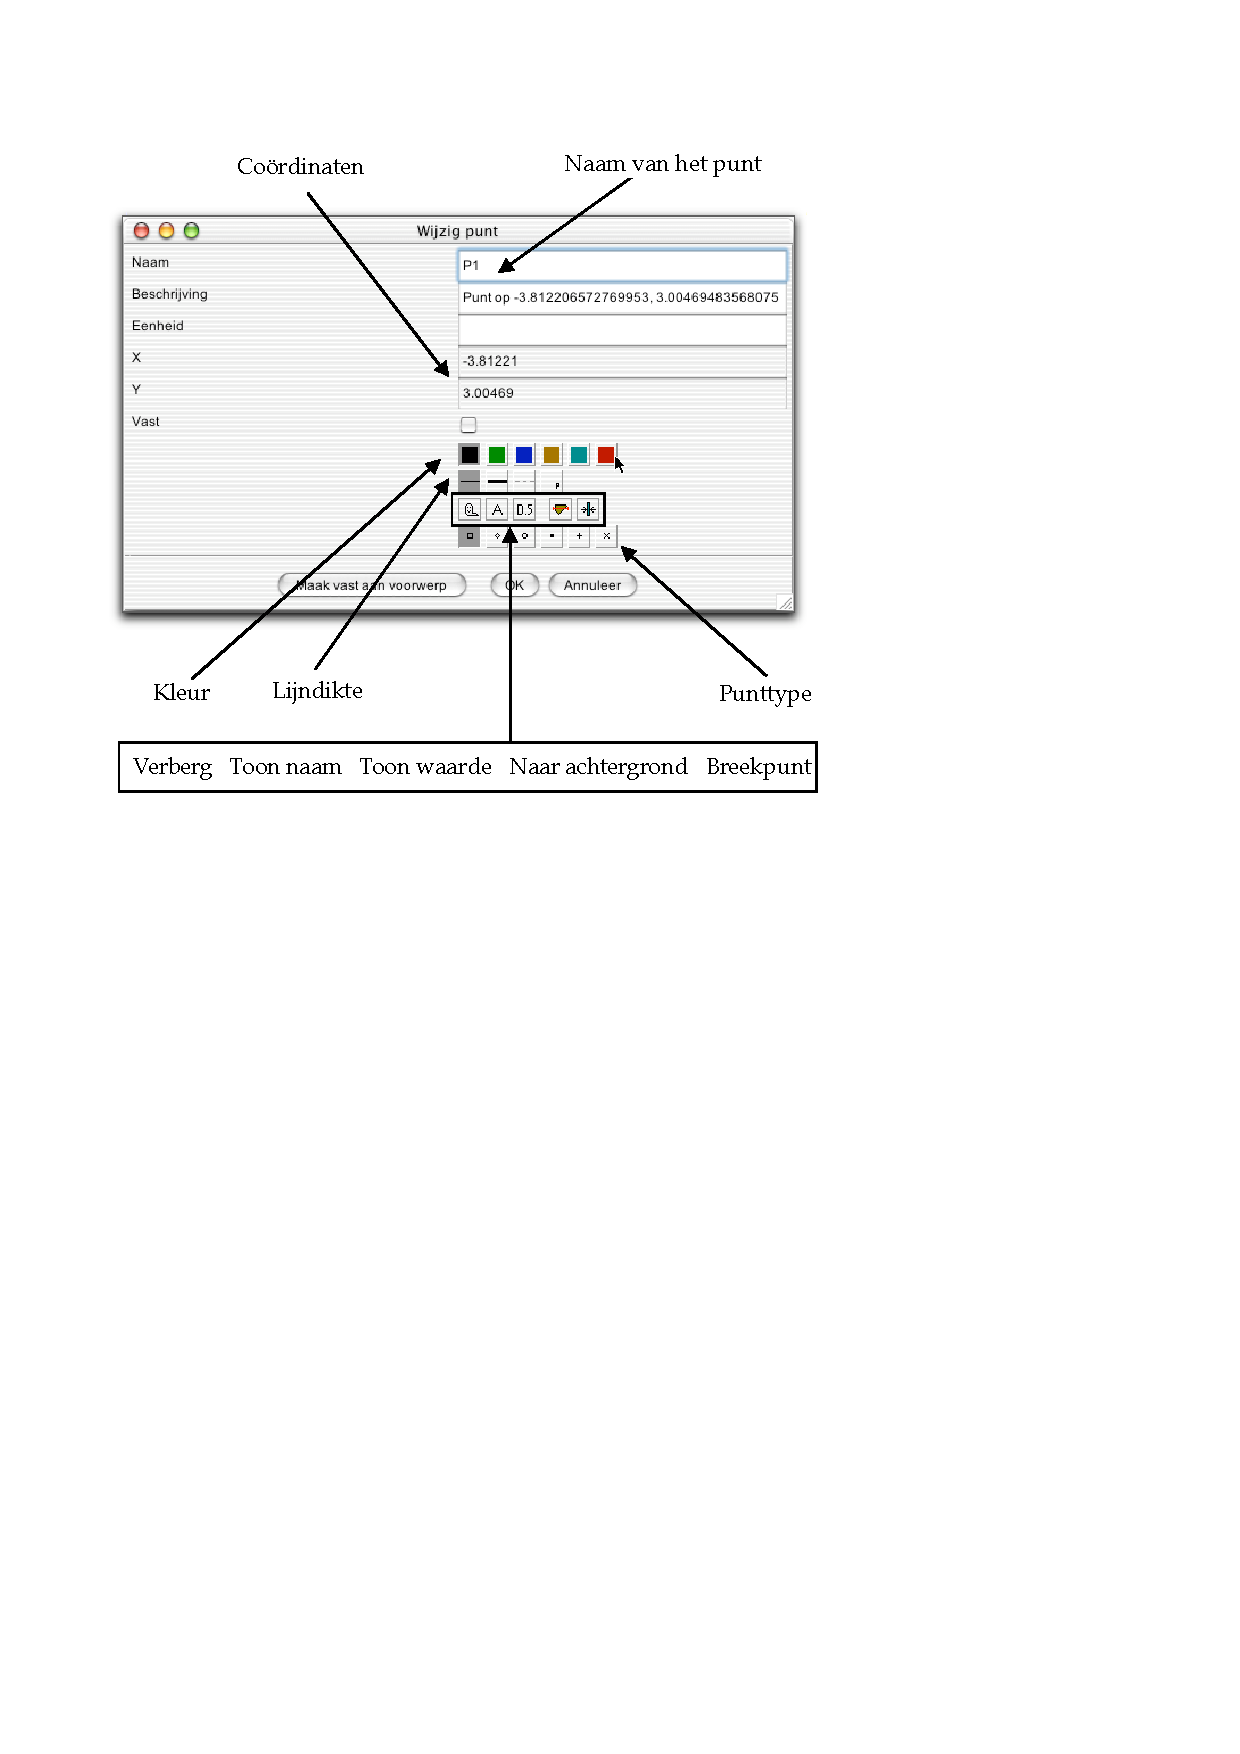
\includegraphics[bb= 42 450 450 780,clip]{figuren/PeL/punteigenschappen.pdf}
       \caption{Eigenschapen van een punt}
    \label{fig:punteig}
\end{figure}

\subsubsection{Benaming -- beschrijving}
P.e.L.\ geeft elk voorwerp een \emph{standaardnaam}. In ons voorbeeld merk je  in het eigenschappenvenster dat punten benoemd worden met een `P' gevolgd door een volgnummer. Bij lijnstukken is dat een `l' met een nummer, snijpunten (intersecties) krijgen  als naam een `I' met een nummer, enz. Voor veel voorwerpen is deze naamgeving prima en is er weinig reden om dat aan te passen.

Voor onze driehoek echter zou het aangenaam zijn als we de `normale' manier van werken zouden kunnen gebruiken: hoekpunten A, B en C. Via het eigenschappendialoogvenster is dat heel simpel. Je klikt in het vakje van de naam en vult de gewenste naam in. Herhaal dit voor de drie punten.

Dit is natuurlijk repetitief werk. Zeker als je de punten van een zeshoek moet benoemen wordt het eentonig. Daarom heeft P.e.L.\ een speciaal commando om dit proces te \emph{automatiseren}: \texttt{Acties$\rightarrow$Hernoem A,B,C} (wat is de sneltoets?).  Het icoon is  niet beschikbaar in de beperkte set werktuigiconen. Je moet deze optie dus uitvinken (\texttt{Instellingen$\rightarrow$Beperkte set werktuigiconen}).
\begin{figure}[htb]
    \centering
    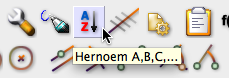
\includegraphics[]{figuren/PeL/herbenoemABC.png}
       \caption{Icoon voor herbenoemen}
    \label{fig:herbenoemicoon}
\end{figure}
Als je dit werktuig kiest, verwacht (zie statusvak!) P.e.L.\ dat je een voorwerp aanklikt. Als je op een punt klikt, zoekt het programma naar de eerste letter die nog niet benomen is, bvb.\ de `A'. Een ander punt aanklikken, levert `B' als benaming, enz. Bij lijnstukken krijg je a, b, c, \dots\ en voor hoeken levert dit $\alpha$, $\beta$, $\gamma$,\dots

Onder de benaming vind je in het dialoogvenster een vak `beschrijving'. Ook hierin komt eens standaardtekst die je kan vervangen door een willekeurige andere tekst. 

\subsubsection{Waarde}
P.e.L.\ laat je blijkbaar toe om vrij in een tekenvenster meetkundige figuren te construeren. Die figuren worden in het programma vertaald in getallen, vergelijkingen, co\"{o}rdinaten. We noemen dit de \emph{waarde} van een voorwerp. Ieder voorwerp heeft zijn specifieke waarde:
\begin{itemize}
\item de waarde van een punt zijn de co\"ordinaten
\item de waarde van een lijnstuk is de lengte
\item de waarde van een cirkel is de  straal
\item de waarde van een hoek is de grootte van de hoek (uitgedrukt in graden)
\end{itemize}
Deze waarde kan je gebruiken in wiskundige uitdrukkingen (\texttt{Acties$\rightarrow$Andere voorwerpen$\rightarrow$Wiskundige uitdrukking}).

 Als je werkt in de permanente instructieweergave (\texttt{Instellingen$\rightarrow$\\Permanente instructieweergave}) kan je de waarde van de voorwerpen gemakkelijk aflezen (zie figuur~\ref{fig:permanent}).
\begin{figure}[htb]
    \centering
    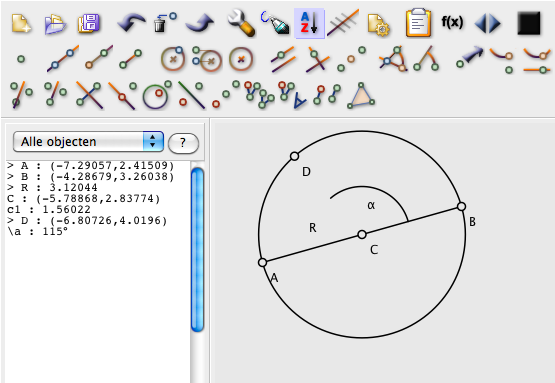
\includegraphics[width=\textwidth]{figuren/PeL/permanente_instructieweergave.png}
       \caption{De permanente instructieweergave}
    \label{fig:permanent}
\end{figure}



\subsubsection{Co\"{o}rdinaten}
Zoals eerder gezegd krijgt elk punt een set van co\"ordinaten. Vaak heb je geen nood aan dit inwendig co\"{o}rdinatensysteem. Voor sommige toepassingen is het wel zinvol dat je met exacte co\"{o}rdinaten werkt. Je kan het raster tonen via het menu \texttt{Opties$\rightarrow$Toon raster} (ga zelf op zoek naar de sneltoets en het bijhorend icoon). Je merkt dat het rastericoon een donkergrijze achtergrond krijgt (met andere woorden: geselecteerd is). Dit is een voorbeeld van een instelling die \emph{voor de hele figuur} van toepassing is (en niet alleen voor een welbepaald voorwerp). 

In het eigenschappenvenster kan je van elk punt de $x$- en de $y$-co\"{o}rdinaat zelf invoeren. Bevestig je keuze en het punt zal opnieuw getekend worden op de co\"{o}rdinaten die je invulde.

Als het raster `aan' staat doen de rasterlijnen dienst als \emph{magneten}. Als je een nieuw punt maakt, wordt dat altijd op een speciale plaats gezet. Experimenteer er maar eens mee. 
In onze constructie brengen de rasterlijnen weinig bij, dus we zetten ze uit. Vooraleer we dat doen, onderzoek je best nog even het effect van de pijltjestoetsen en van de `+' en de `-' toetsen. Soms is een figuur te klein of te groot, of valt ze een stuk buiten het venster. Met deze toetsen kan je de figuur verkleinen of vergroten en verschuiven\footnote{Eigenlijk is dat niet echt correct geformuleerd. De figuur blijft staan, maar het onderliggend co\"{o}rdinatensysteem wordt aangepast. Je kan het ook als volgt bekijken. De constructie wordt op een heel groot blad papier gemaakt. Jij krijgt enkel een klein stuk van dat tekenpapier te zien, door een venster. Dit venster kan je verschuiven over het tekenblad en je kan er een vergrootglas (of verkleinglas) voor zetten.}.

Maar ---\,zoals gezegd\,--- we zetten het rastersysteem af voor de rest van onze constructie.

\subsubsection{Visuele kenmerken}
We gaven het hiervoor al aan. Bepalend voor het eindresultaat is zeker en vast ook een \emph{oordeelkundig gebruik van kleur, puntsoort, lijndikte, naamgeving,...}

In het eigenschappenvenster kan je voor elk voorwerp apart deze eigenschappen instellen. Experimenteer met deze instellingen. Je kan eigenlijk niets fout doen en de meeste dingen zijn voor de hand liggend.

Alleen de `Verberg' optie vraagt een woordje uitleg. Deze mogelijkheid om voorwerpen niet te laten zien op het scherm ---\,ook al zijn ze wel nog aanwezig in de constructie\,--- is absoluut onmisbaar voor meer \emph{complexe constructies}. Tenzij je heel wat tussenstappen onzichtbaar maakt, zie je op den duur door de bomen het bos niet meer. 

Op zich is het een simpele optie. Je duidt bij een voorwerp bij de eigenschappen aan dat het verborgen mag worden. Als je je later zou bedenken, kan je het `verberg' icoontje `uit' zetten. Het probleem is natuurlijk dat je moeilijk een voorwerp kan selecteren (door er rechts op te klikken) dat je niet meer kan zien. De oplossing vind je in het menu: \texttt{Opties$\rightarrow$Toon verborgen voorwerpen} (zoek de sneltoets: bij langere constructies zal je die regelmatig nodig hebben). Net zoals bij het raster is dit ook een optie die voor heel de constructie geldig is, tot je ze uitzet. Verborgen voorwerpen worden in een lichte tint getekend. Je kan nu de eigenschappen van het verborgen voorwerp dat je weer wil tonen, wijzigen (bvb.\ door rechtsklikken). Zet in het eigenschappendialoogvenster de optie `verberg' uit. Je kan nu in het menu \texttt{Opties$\rightarrow$Toon verborgen voorwerpen} terug uitzetten.



\subsection{Midden van de drie zijden}
Na de (toch wel belangrijke) uitwijding hierboven keren we terug naar ons voorbeeld. We hebben al de driehoek getekend en de drie hoekpunten A, B en C genoemd. Deze namen zijn zichtbaar op de constructie. De namen van de lijnstukken worden niet getoond.

Volgende stap: middelloodlijnen tekenen. Er is weliswaar een `middelloodlijn' werktuig\footnote{Perpendicular Bisector 
\includegraphics[width=0.75cm]{figuren/PeL/middelloodlijnicoon.png}}, maar daar gaan we geen gebruik van maken. We werken daarom in twee stappen en zoeken eerst de middens van de zijden. 

Het verhaal ken je stilaan. Je selecteert het `midden' werktuig (via het menu, via een icoon of via een sneltoets) en werpt een blik op het statusvak linksonder. Als daarin de tekst `Middelpunt: eerste punt?' verschijnt, zit je goed. 

Dit keer proberen we slim te zijn. \emph{Vooraleer} de middens te construeren, denken we even na hoe we die getoond willen zien. Nemen we bvb.\ dat we ze in het rood, met een bolletje en voorzien van de standaardbenaming willen tonen. Hierboven zag je reeds hoe je na de constructie nog eigenschappen kan veranderen. Als je echter op voorhand weet wat je wil, is het effici\"{e}nter om het op voorhand te bepalen. 

In wat volgt werken we via het menu. Ook hier kan je de selectie via de iconen doen. Denk er wel aan dat deze instellingen blijven gelden voor alle voorwerpen die je vanaf nu construeert. Kies in het menu achtereenvolgens volgende instellingen:
\begin{itemize}
\item \texttt{Opties$\rightarrow$Standaard kleur$\rightarrow$rood}
\item \texttt{Opties$\rightarrow$Standaard punttype$\rightarrow$Cirkel}
\item \texttt{Opties$\rightarrow$Voorkeuren$\rightarrow$Toon voorwerpnamen}
\end{itemize}
De andere instellingen laten we zoals het is. Merk je in de iconenbalk wat er veranderd is? Construeer nu de middens van de drie zijden.

\subsection{Loodlijnen}
We willen de drie loodlijnen graag in een blauwe stippellijn tekenen. De namen willen we er liever niet bij. Pas de opties in die zin aan. Zoek zelf het loodlijn gereedschap. Kijk in de statusbalk wat P.e.L.\ van jou verwacht. De volgorde van de invoer is belangrijk: moet je eerst de rechte aanduiden en dan het punt of is het omgekeerd? 


\section{Opbouw van een constructie}
Het boeiende aan programma's zoals P.e.L.\ is dat je de zogenaamde \emph{vrije punten} van de constructie kan verplaatsen. De tekening past zich dan aan aan de nieuwe situatie. We noemen dit het \emph{dynamisch} of het \emph{interactief} karakter van dit soort van meetkundeprogramma's. 

In P.e.L.\ kan je \emph{enkel punten} verplaatsen. Het verschil tussen vrije en niet-vrije punten is in dit opzicht belangrijk. In ons voorbeeld zijn de drie hoekpunten van de driehoek vrije punten. Het zijn punten die we willekeurig ergens in het tekenvenster geplaatst hebben\footnote{Hadden we de Shift-toets ingedrukt gehouden bij het cre\"{e}ren van de punten, dan waren dit vaste punten geweest.}. Een vrij punt kan je met het `beweeg' werktuig verplaatsen. Dit werktuig kan je op de gebruikelijke manieren selecteren, bvb.\ via de sneltoets `b' (zoek zelf hoe je het doet met een icoon of via het menu!). Als je dit werktuig geselecteerd hebt, krijg je feedback van het programma via de statusbalk en via het tekenvenster. Alle vrije (beweegbare) punten worden immers \emph{rood gekleurd} en in het \emph{vet} weergegeven. Klik op zo'n punt, hou de muisknop ingedrukt en verplaats het punt. De hele constructie past zich aan. Tip: \emph{als je de Ctrl-toets ingedrukt houdt, blijf je de originele tekening zien}.

De middelpunten van de zijden zijn \emph{geen} vrije punten. Hun plaats ligt vast, want ze volgt uit een berekening waar twee vrije punten de invoerparameters zijn. 

Tijdens de constructie maak je onvermijdelijk ooit wel eens een \emph{fout}. Als je het laatst geconstrueerde voorwerp wil wissen is het vrij eenvoudig: \texttt{Acties$\rightarrow$ Wis laatste voorwerp}. Onthoud misschien best ook de sneltoets voor deze bewerking. Je zal immers regelmatig wel eens iets moeten wissen.

Als je \emph{pas na een aantal stappen} merkt dat je in het begin een fout maakte, wordt het iets moeiljker. Je gebruikt hiervoor \texttt{Acties$\rightarrow$Verwijder voorwerp en zijn kinderen}. De klemtoon bij deze actie ligt echt wel op `en zijn kinderen'. Als je in onze driehoek \'{e}\'{e}n van de hoekpunten verwijdert, valt een groot deel van de constructie mee weg (ga eens na wat er allemaal van dit ene punt afhangt). Kalm blijven is de boodschap! Denk eerst eens goed na of je wel het goede voorwerp wil wissen. Als het dan toch fout loopt (en je bent een groot deel van je constructie kwijt) is `\texttt{Acties$\rightarrow$Maak wissen ongedaan' (Ctrl-Z)} je bondgenoot. \emph{Voorwaarde is wel dat je na je fatale wisbewerking geen andere bewerkingen meer deed}. 

Zoals bij elk computerprogramma neem je natuurlijk je voorzorgen en bewaar je je werk regelmatig. 

\section{De omcirkel}
Hoe je ook de driehoek aanpast (door punten te verplaatsen), de middelloodlijnen op de drie zijden gaan altijd door \'{e}\'{e}n punt. Dit snijpunt ligt even ver van de drie hoekpunten verwijderd. We kunnen met andere woorden een cirkel tekenen die door de drie hoekpunten van de gegeven driehoek gaat, met als middelpunt het snijpunt van de middelloodlijnen.

\emph{Werken met snijpunten} is anders in dit soort van programma's dan bij een constructie op papier. Als je op papier twee snijdende rechten tekent met een potlood, heb je automatisch een snijpunt. Bij programma's voor dynamische meetkunde moet je dit snijpunt meestal expliciet aangeven, vooraleer je het kan gebruiken\footnote{Dit is een vereenvoudiging van hoe je in P.e.L.\ werkt. Het kan ook zonder dit punt expliciet te benoemen, maar we leggen hier de standaardmanier van werken uit}. Om snijpunten te construeren beschik je over een apart gereedschap: het `intersectie' werktuig.

Kies dit werktuig. In de statusbalk merk je dat er verschillende mogelijkheden zijn om het snijpunt te construeren:
\begin{enumerate}
\item Je kan de verschillende snijdende voorwerpen \'{e}\'{e}n voor \'{e}\'{e}n selecteren.
\item Je kan echter ook rechtstreeks op het snijpunt klikken. Soms is dit niet mogelijk omdat je bvb.\ \emph{alle} snijpunten wilt (bvb.\ tussen een rechte en een cirkel) of omdat het snijpunt heel dicht bij andere punten ligt.
\end{enumerate}
Hier kan je kiezen welke methode je gebruikt. Construeer het snijpunt.

Om een cirkel te construeren zijn er verschillende mogelijkheden:
\begin{itemize}
\item Cirkel met gegeven middelpunt en een punt op de cirkel;
\item cirkel met gegeven middelpunt  en nog twee andere punten die de straal bepalen;
\item cirkel met gegeven middelpunt en een in te voeren lengte als straal.
\end{itemize}
De keuze hangt af van de omstandigheden. Voor deze constructie ligt de eerste optie voor de hand. De statusbalk helpt je wel verder bij de juiste keuze van de punten (eerst het middelpunt selecteren, en dan \'{e}\'{e}n van de hoekpunten van de driehoek).


\section{Constructievoorbeelden stap voor stap}
\subsection{Vierkant}
\begin{quote}
Teken een vierkant $ABCD$ met een willekeurige zijde.
\end{quote}
\begin{figure}
\begin{center}
\setlength{\fboxrule}{0.4pt}
\setlength{\fboxsep}{0.1pt}
\framebox{
\setlength{\unitlength}{0.008466666666666667cm}
\begin{picture}(1181.0,708.0)
\put(0,0){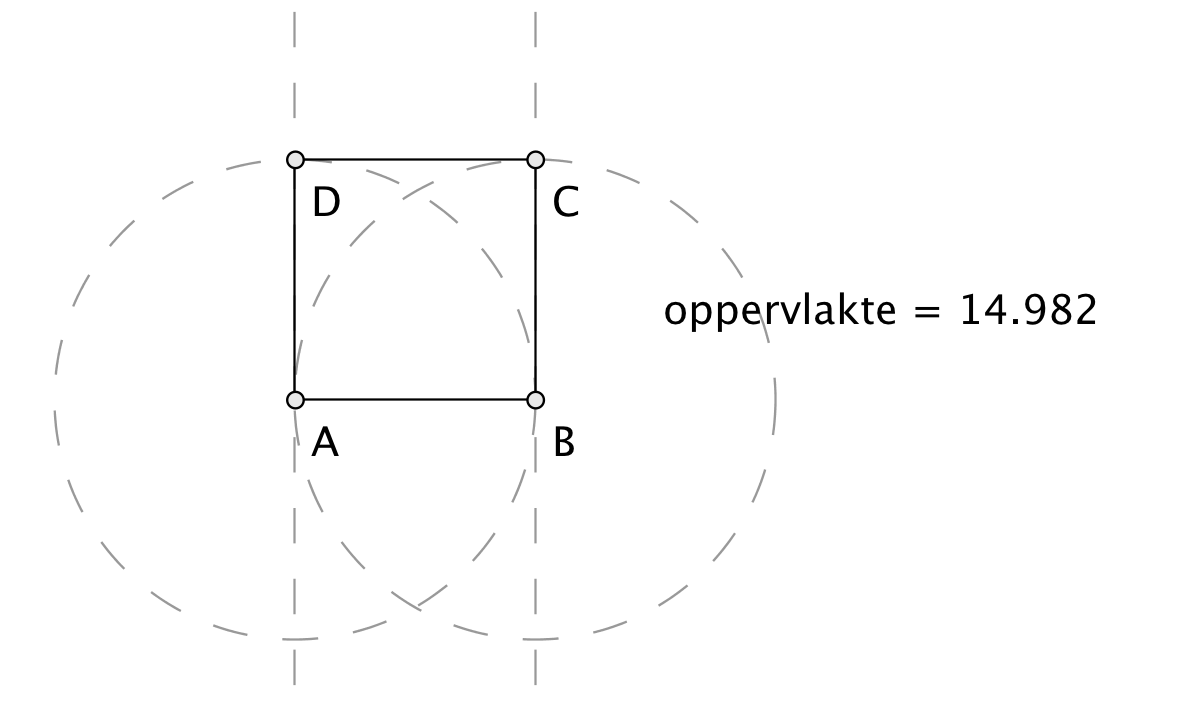
\includegraphics[width=9.999cm]{figuren/PeL/vierkant.png}}
\put(403.072,343.191){$a$}
\put(243.646,413.511){$d$}
\put(404.072,583.438){$c$}
\put(560.499,413.511){$b$}
\end{picture}
}
\end{center}
\caption{Constructie van een vierkant}
\label{fig:vierk}
\end{figure}
\begin{enumerate}
\item Teken de punten $A$ en $B$. Gebruik het werktuig \knop{Hernoem A,B,C} om de punten de correcte naam te geven.
\item Verbind beide punten met een lijnstuk. Benoem het lijnstuk $a$.
\item Construeer nu de rechteropstaande zijde als volgt:
\begin{enumerate}
\item Maak een loodrechte op $a$ door het punt $B$ in stippellijn.
\item Teken in stippellijn een cirkel met middelpunt $B$ en straal gelijk aan de lengte van $a$. Je gebruikt daarvoor het werktuig \knop{Cirkel met straal r en middelpunt M}. Volg de instructies van de instructiebalk nauwkeurig op. Het beginpunt van de straal is het punt $A$ en het eindpunt $B$.
\item Bepaal het snijpunt van de cirkel en de loodrechte met het werktuig \knop{Intersectie}. Verander eerst de lijndikte.
\item Benoem het bovenste snijpunt $C$ en verwijder het andere snijpunt met \knop{Verwijder voorwerp en zijn kinderen}.
\item Teken het lijnstuk $BC$. Benoem de zijde $b$.
\end{enumerate}
\item Construeer nu de linkeropstaande zijde $AD$ op dezelfde manier als $BC$ en benoem hem $d$.
\item Teken het lijnstuk $CD$ en noem het $c$.
\end{enumerate}

Je hebt nu het vierkant $ABCD$ getekend. Je kan de lengte van de zijde van het vierkant wijzigen door de punten $A$ of $B$ te slepen met het werktuig \knop{Beweeg punt}. Merk op dat de punten $C$ en $D$ niet vastgenomen (om ze te verslepen) kunnen worden. Zij zijn immers {\it vaste punten}: ze zijn het resultaat van een aantal bewerkingen.

De tekening wordt eleganter als je de hulplijnen verbergt (niet verwijderen!). Je kan ze op de achtergrond zichtbaar maken met \knop{Toon verborgen voorwerpen}.

Bewaar je afbeelding. Verwijder dan het punt $A$. Wat merk je? Zoek een verklaring.

Veronderstel dat we ook de oppervlakte van het vierkant willen tonen op het scherm. Daarvoor gebruiken we het  werktuig \knop{Wiskundige uitdrukking}. Als je op de knop klikt, krijg je het dialoogvenster zoals in figuur~\ref{fig:wisk_uitdr}.
\begin{figure}
\centering
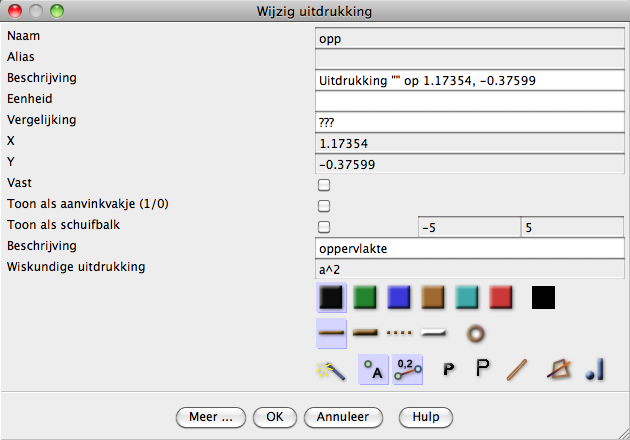
\includegraphics[width=\textwidth]{figuren/PeL/wisk_uitdrukking.png}
\caption{Dialoogvenster van het werktuig `Wiskundige uitdrukking'}
\label{fig:wisk_uitdr}
\end{figure}
\begin{enumerate}
\item Een wiskundige uitdrukking is een voorwerp, net zoals een cirkel, en heeft dus een naam en een waarde. Met de naam (hier `opp') kan je de waarde oproepen in een ander voorwerp (bijvoorbeeld bij een cirkel met vaste straal). 
\item Vul het onderste veld \knop{Beschrijving} in met \veld{oppervlakte}.  Deze tekst verschijnt bij de tekening (zie afbeelding~\ref{fig:vierk}). 
\item Bij \knop{Wiskundige uitdrukking} vul je de waarde in die je wil bekomen, namelijk het kwadraat van het lijnstuk $a$. Je kan dit doen op twee manieren: ofwel vul je gewoon \verb/a^2/ in (de waarde van het lijnstuk $a$ is immers zijn lengte), ofwel gebruik je de functie \veld{d(A,B)} waarbij je de afstand tussen de punten $A$ en $B$ berekent. \item Vink zowel \knop{Toon voorwerpnamen} als \knop{Toon voorwerpwaarden} aan.
\end{enumerate}
Met het werktuig \knop{Wiskundige uitdrukking} kan je ook een voorwerp maken waarvan de waarde bepaald wordt door middel van een schuifbalk. Je vult het veld `Wiskundige uitdrukking' niet in, maar je vinkt het vakje 'Toon als schuifbalk' aan. In de figuur verschijnt dan een schuifbalk. Door het punt op de schuifbalk te verschuiven, wijzig je de waarde van het voorwerp.

\subsection{Lindenmayer-fractaal}
De Lindenmayer-fractaal ziet er als volgt uit:
\begin{center}
\setlength{\fboxrule}{1.pt}
\setlength{\fboxsep}{0.1pt}
\scalebox{0.4}{\framebox{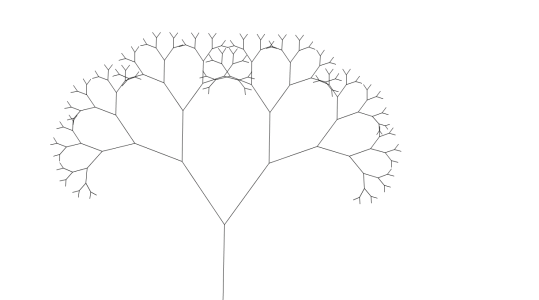
\includegraphics{figuren/PeL/lindmayer.png}}}
\end{center}

Ze wordt iteratief opgebouwd. Dit wil zeggen: je vertrekt van een stam en daar teken je twee takken op. Vervolgens beschouw je elk van deze takken opnieuw als stam en teken je telkens twee (kleinere) takken. De verhouding van de lengte tak - onderliggende tak moet telkens gelijk zijn.
\begin{center}
\setlength{\fboxrule}{1.pt}
\setlength{\fboxsep}{0.1pt}
\scalebox{0.5}
{\framebox{
\setlength{\unitlength}{0.008466666666666667cm}
\begin{picture}(1417.0,929.0)
\put(0,0){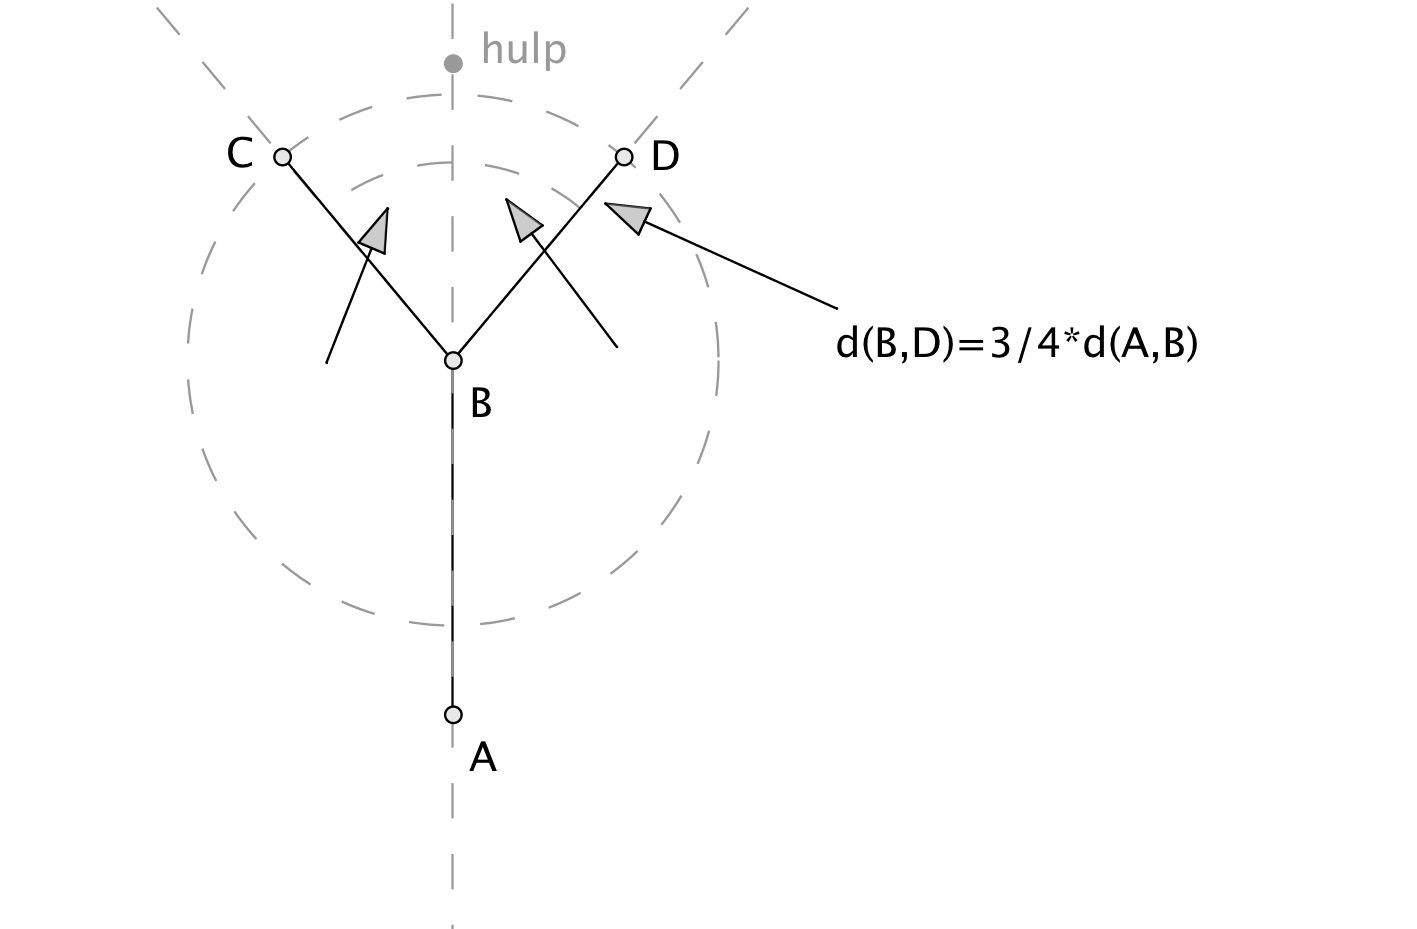
\includegraphics[width=11.997cm]{figuren/PeL/flower.png}}
\put(390.07,121.222){$r_1$}
\put(245.424,516.593){$\alpha=40^\circ$}
\put(576.436,527.929){$\beta=40^\circ$}
\end{picture}
}}
\end{center}
De constructie is wat moeilijker en maakt gebruik van macro's. We beginnen met het tekenen van een stam en zijn twee takken.

\begin{enumerate}
\item Construeer het \knop{lijnstuk} $a$ van $A$ tot $B$.
\item Maak in stippellijn de \knop{rechte} $r_1$ door $A$ en $B$.
\item Definieer een \knop{punt} \veld{hulp} op deze rechte, ten noorden van $B$.
\item Construeer de \knop{vaste hoeken} $\alpha$ en $\beta$ van $40^\circ$ met \knop{beginpunt} \veld{hulp} en \knop{basispunt} $B$\footnote{Let op de volgorde! Indien je straks problemen hebt bij de macro, kom dan terug naar deze stap.}. \label{voetnoot_lindmayer}
\item Construeer in stippellijn de \knop{cirkel} $c_1$ \knop{met vaste straal}  \veld{3/4*d(A,B)} en middelpunt $B$.
\item Bepaal de snijpunten $C$ en $D$ van deze cirkel met de hoeken $\alpha$ en $\beta$ respectievelijk.
\item Teken de lijnstukken $BC$ en $BD$. Deze lijnstukken zijn de takken op de stam $AB$.
\end{enumerate}

In feite heb je nu de eerste iteratie van de fractaal getekend. Een fractaal met \'e\'en iteratie is echter geen fractaal. Op {\it beide} takken die je getekend hebt, zou je nu opnieuw de ganse constructie moeten hernemen. Dit geeft vier (kleinere) takken, waarop je opnieuw takken moet maken \dots\ Het zal een werk van zeer lange adem zijn.

Het is bijgevolg beter een {\it macro} te maken. Een macro is in feite een samenraapsel van een aantal opeenvolgende constructies. Eens hij gedefinieerd is, volstaat het \'e\'en of meerdere beginpunten of -voorwerpen ({\knop{parametervoorwerpen}) aan te duiden. De macro zorgt er dan voor dat het eindresultaat (\knop{doelvoorwerpen}) getekend worden.

We maken nu de macro {\tt lindenmayer} die de stam $AB$ als {\knop{parametervoorwerp} heeft en de takken $BC$ en $BD$ als \knop{doelvoorwerpen}. We gebruiken hiertoe bovenstaande constructie.

\begin{enumerate}
\item Klik op de knop \knop{Macro parameters/doelen/definitie}.
\item P.e.L.\ vraagt \knop{Macro parameters: parametervoorwerpen?}. Dit zijn de gegevens waarop het uiteindelijke resultaat van je macro gebaseerd zijn. Hier heb je twee mogelijkheden: je zou de punten $A$ en $B$ kunnen aanklikken, maar ook het lijnstuk $AB$ (dat op deze punten gedefinieerd is). Wij kiezen voor de laatste mogelijkheid.
\item \label{lindmayer: stap 3} Klik opnieuw op de knop \knop{Macro parameters/doelen/definitie}. Merk op dat de knop verandert, en dat een deel van de constructie verdwijnt\footnote{Dit is niet abnormaal. Indien echter de takken $BC$ en $BD$ ook verdwijnen, heb je de constructie verkeerd gemaakt. Lees opnieuw de voetnoot op blz.~\pageref{voetnoot_lindmayer}.}. P.e.L.\ vraagt nu \knop{Macro doelen: doelvoorwerpen?}. Wat moet het resultaat zijn van je macro? Wij willen dat de macro twee takken op de stam $AB$ tekent, dus we klikken de lijnstukken $BC$ en $BD$ aan.
\item Klik een laatste keer op de knop \knop{Macro parameters/doelen/definitie}. P.e.L.\ vraagt je nu de \knop{naam} van de macro te specifi\"eren. Verder kan je de macro van commentaar voorzien en in het veld \knop{Vraag naar parameters} een zinvolle naam invullen (bijvoorbeeld \veld{stam} in plaats van het standaard voorziene $l_1$).
\item Klik op OK en je macro is klaar.
\end{enumerate}

Misschien lukte bovenstaande procedure niet omdat in stap~\ref{lindmayer: stap 3} je scherm opeens leeg was. De oorzaak hiervan ligt in een foute constructievolgorde. De doelvoorwerpen moeten {\it volledig} afhankelijk zijn van de parametervoorwerpen. Je mag bijvoorbeeld de hoek van $40^\circ$ niet defini\"eren op een rechte die niet door $A$ en $B$ gaat (maar wel door twee andere punten op het lijnstuk $AB$). Op zicht zal je dezelfde takken krijgen, maar voor P.e.L.\ maakt het een groot verschil: de takken zijn immers afhankelijk van de nieuwe punten, en niet van $A$ en $B$. V\'o\'or je een macro begint zou je de volgende test moeten doen: verwijder de parametervoorwerpen\footnote{Eerst constructie opslaan!}. Indien de doelvoorwerpen niet verdwijnen, is de constructievolgorde fout en zal je ook geen macro kunnen defini\"eren.

Nu je de macro gemaakt hebt, kan je hem gebruiken.
\begin{enumerate}
\item Klik rechts op het scherm en selecteer de macro.
\item P.e.L.\ vraagt je naar het parametervoorwerp \veld{stam}. Klik op een tak waar je zijtakken wil.
\item De zijtakken worden getekend.
\end{enumerate}
Het kan zijn dat je een foutief resultaat krijgt, bijvoorbeeld dat de nieuwe takken naar beneden wijzen in plaats van naar boven. Dit is opnieuw te wijten aan een foute constructievolgorde (bijvoorbeeld het lijnstuk $AB$ construeren van $B$ naar $A$ in plaats van $A$ naar $B$. Er is maar \'e\'en oplossing: opnieuw beginnen met de volledige constructie en nu de juiste volgorde aanhouden.


 